\documentclass[../../main.tex]{subfiles}

\graphicspath{{../../image/}{../../figure/}}

\begin{document}

\section{对抗训练}\label{section:ch17-对抗训练}

考虑一个基于从潜空间 $z$ 到数据空间 $x$ 的非线性变换的生成式模型。引入一个潜空间分布 $p(z)$，它可能是一个简单的 Gauss 分布：
\begin{align}
p(z)=\mathcal{N}(z\mid\bm{0},\bm{I}).
\label{align:ch17-潜空间分布}
\end{align}

同时定义一个由深度神经网络实现的非线性变换 $x=g(z,w)$，其中可学习参数 $w$ 对应的网络称为\textbf{生成器}（generator）网络。它们共同隐式地定义了 $x$ 上的分布，我们的目标是将这个分布拟合到一组训练样本 $\{x_n\}$ 上，其中 $n=1,\cdots,N$。然而，我们并不能通过优化似然函数来确定 $w$，因为这通常无法以封闭形式来计算。生成对抗网络（Goodfellow et al., 2014; Ruthotto and Haber, 2021）的关键思想是引入判别器（critic）网络，判别器网络与生成器网络一起训练，并为更新生成器的权重提供训练信号，如\cref{figure:ch17-GAN示意图}所示。

\begin{figure}[htbp]
  \centering
  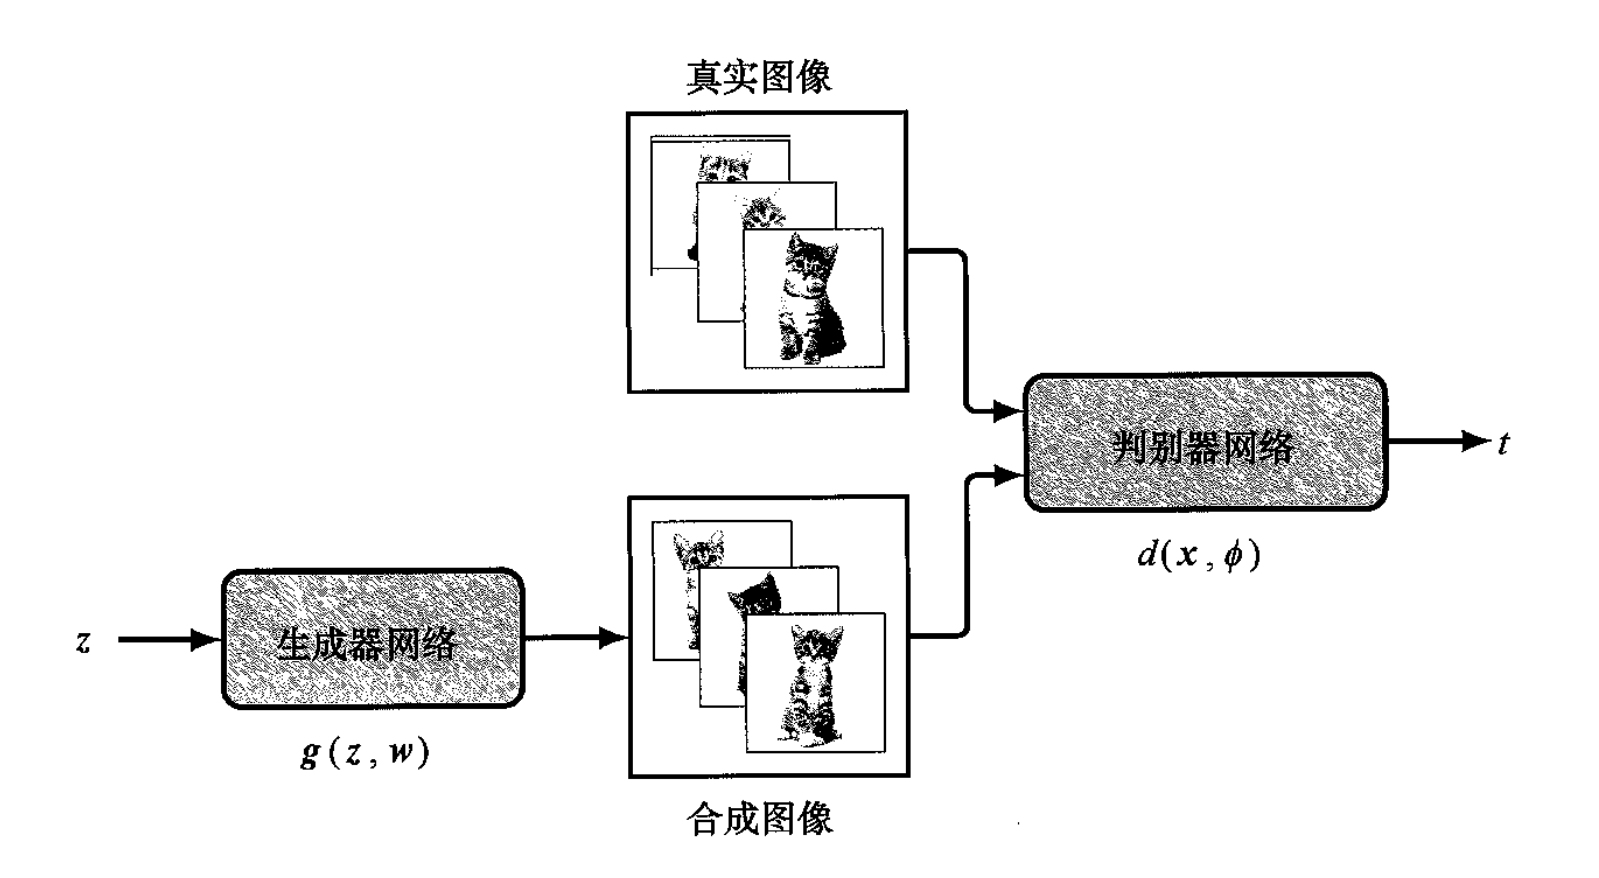
\includegraphics[width=0.82\textwidth]{ch17-fig484-gan-schematic.png}
  \caption{生成对抗网络的示意图。在这样的网络中，训练判别器网络 $d(x,\phi)$ 以区分来自训练集的真实样本（小猫的图像）和由生成器网络 $g(z,w)$ 产生的合成样本。生成器网络的目标是通过产生逼真的图像来让判别器网络产生更多的误判，而判别器网络的目的是通过更好地区分真实样本和合成样本来减少误判}
  \label{figure:ch17-GAN示意图}
\end{figure}

\begin{definition}[生成对抗网络]\label{definition:ch17-生成对抗网络}
设 $p(z)$ 是潜空间上的给定分布，$g(\cdot,w)$ 是参数为 $w$ 的深度神经网络。称 $g(\cdot,w)$ 为\textbf{生成器}（generator）网络。由 $z\sim p(z)$ 与 $x=g(z,w)$ 共同决定的 $x$ 上的分布称为\textbf{生成分布}，记作 $p_g(x)$。称参数为 $\phi$ 的网络 $d(\cdot,\phi)$ 为\textbf{判别器}（critic）网络，它把数据向量 $x$ 映射为 $x$ 来自真实数据（而不是来自生成分布）的概率。判别器网络与生成器网络一起训练、互为对手，这一训练方式称为\textbf{对抗训练}（adversarial training）。
\end{definition}

% SUPPLEMENT: parent=definition:ch17-生成对抗网络; kind=motivation; location=紧随其后的 remark（重构新增）
\begin{remark}（重构新增）
这里把生成式模型写成“先取 $z\sim p(z)$、再作确定性变换 $x=g(z,w)$”的形式，动机是绕开似然函数。GAN 并不要求能写出 $p_g$ 的密度，只要求能从 $p(z)$ 采样并把样本经 $g$ 推送出去；因此它是隐式（implicit）的生成式模型，与\cref{chapter:ch16-连续潜变量}中以 $p(x\mid z,w)$ 的可求值为前提的非线性潜变量模型有本质区别：后者通过最大化边缘似然来学习，前者通过判别器提供的信号来学习。

定义中的每一项都有作用。$p(z)$ 被固定为一个简单分布（如\eqref{align:ch17-潜空间分布}的标准 Gauss 分布），是把全部建模负担交给 $g$ 的刻意选择：若 $p(z)$ 也可学，则它与 $g$ 的重参数化不唯一，模型不可识别。$g$ 关于 $w$ 的可微性是训练的前提，因为生成器的梯度要经由 $g$ 反传到 $w$。判别器输出必须落在 $(0,1)$ 内，才能与\eqref{align:ch17-判别器输出}的概率解释相容，并保证对数损失有定义。

最后要强调，$p_g$ 一般没有关于 Lebesgue 测度的密度：当 $z$ 的维数低于 $x$ 的维数时，$p_g$ 集中在 $g$ 的像（一个低维流形）上。这正是理论分析中必须额外假定 $p_g$ 与 $p_{\mathrm{data}}$ 处处有正密度的原因，见\cref{proposition:ch17-最优判别器}。
\end{remark}

判别器网络的目标是区分来自数据集的真实样本和由生成器网络的合成（或“假”）样本，它通过最小化传统的分类误差函数来进行训练。相反，生成器网络的目标是通过生成与训练集同分布的样本来最大化这个误差。因此，生成器网络和判别器网络互相对抗，“生成对抗网络”由此得名。

\begin{definition}[零和博弈]\label{definition:ch17-零和博弈}
设两个参与者分别以 $w$ 与 $\phi$ 为策略，其收益分别为 $E(w,\phi)$ 与 $-E(w,\phi)$。若一个参与者的收益恰好是另一个参与者的损失，即两个收益之和恒为零，则称这样的博弈为\textbf{零和博弈}（zero-sum game）。
\end{definition}

% SUPPLEMENT: parent=definition:ch17-零和博弈; kind=motivation; location=紧随其后的 remark（重构新增）
\begin{remark}（重构新增）
把对抗训练看作零和博弈，是为了给“谁进步了”确立一个共同的标尺：若双方的收益之和不为零，就存在对双方都有利的方向，对抗性随之消失，“生成器变强必然使判别器变难”这一直观也不再成立。零和性还保证整个训练只有一个标量目标 $E(w,\phi)$，于是\eqref{align:ch17-判别器更新}与\eqref{align:ch17-生成器更新}只是同一函数上的两个相反方向。

需要区分两件事：零和是对训练目标的建模假设，而收敛是动力学性质。博弈为零和并不意味着梯度下降-上升一定收敛到鞍点；恰恰相反，\cref{exercise:ch17-02}将给出一个零和目标 $E(a,b)=ab$ 的例子，其梯度动力学绕鞍点作周期运动而永不收敛。
\end{remark}

生成对抗网络通过允许判别器网络提供一个训练信号来训练生成器网络，从而将无监督的密度建模问题转换成了一种监督学习的形式。

\subsection{损失函数}\label{subsection:ch17-损失函数}

为了明确这一点，我们定义一个二元目标变量 $t$：
\begin{align}
t=1,&\quad\text{代表真实数据}\label{align:ch17-t真实}\\
t=0,&\quad\text{代表合成数据}\label{align:ch17-t合成}
\end{align}

判别器网络拥有单个输出单元，带有 sigmoid 激活函数，其输出表示数据向量 $x$ 为真实数据的概率：
\begin{align}
P(t=1)=d(x,\phi).
\label{align:ch17-判别器输出}
\end{align}

我们可以使用如下标准的交叉熵损失函数来训练判别器网络：
\begin{align}
E(w,\phi)=-\frac{1}{N}\sum_{n=1}^{N}\Big\{t_n\ln d_n+(1-t_n)\ln(1-d_n)\Big\},
\label{align:ch17-交叉熵}
\end{align}
其中 $d_n=d(x_n,\phi)$ 是判别器网络的输出，我们已经通过数据点的总数对它进行了归一化（参见\cref{subsection:ch01-模型复杂度}）。训练集包括标记为 $x_n$ 的真实样本和由生成器网络 $g(z_n,w)$ 输出的合成样本，其中 $z_n$ 是从潜空间分布 $p(z)$ 中采样的随机样本。对于真实样本，$t_n=1$；对于合成样本，$t_n=0$。我们可以将损失函数［\eqref{align:ch17-交叉熵}］写成以下形式：
\begin{align}
E_{\mathrm{GAN}}(w,\phi)={}&-\frac{1}{N_{\mathrm{real}}}\sum_{n\in\mathrm{real}}\ln d(x_n,\phi)\nonumber\\
&-\frac{1}{N_{\mathrm{synth}}}\sum_{n\in\mathrm{synth}}\ln\big(1-d(g(z_n,w),\phi)\big).
\label{align:ch17-GAN损失}
\end{align}

通常情况下，真实数据点的数量 $N_{\mathrm{real}}$ 等于合成数据点的数量 $N_{\mathrm{synth}}$。这种生成器网络和判别器网络的组合可以使用随机梯度下降进行端到端的训练（参见\cref{chapter:ch07-梯度下降}），并通过反向传播来计算梯度。然而，这种训练方式的独特之处在于其对抗性，即误差相对于 $\phi$ 最小化，而相对于 $w$ 最大化。

这种最大化可以通过标准的基于梯度的方法来完成，通过反转梯度的符号，参数更新为
\begin{align}
\Delta\phi&=-\lambda\nabla_\phi E_n(w,\phi),\label{align:ch17-判别器更新}\\
\Delta w&=\lambda\nabla_w E_n(w,\phi),\label{align:ch17-生成器更新}
\end{align}
其中 $E_n(w,\phi)$ 表示为数据点 $n$ 定义的误差，或者更一般地说，是为小批量数据点定义的误差。注意\eqref{align:ch17-判别器更新}和\eqref{align:ch17-生成器更新}右侧的符号不同，因为判别器网络的训练目标是降低错误率，而生成器网络的训练目标是提高错误率。实际上，训练交替地在更新生成器网络的参数和更新判别器网络的参数之间进行，每次只使用一个小批量数据，并采取一个梯度下降步骤，之后生成一组新的合成样本。

如果生成器网络成功找到完美解决方案，则判别器网络将无法区分真实数据和合成数据，因此其输出始终为 $0.5$。一旦 GAN 训练完毕，判别器网络就会被舍弃，生成器网络则用来从潜空间中采样并将这些样本经训练好的生成器网络加以传播，从而在数据空间中合成新的样本。我们可以证明，对于具有无限灵活性的生成器网络和判别器网络，完全优化的 GAN 将具有与数据分布完全匹配的生成分布（见\cref{exercise:ch17-01}）。\cref{figure:ch01-生成人脸}展示了一些由 GAN 生成的优秀的人脸图像。

到目前为止我们所讨论的 GAN 都是从无条件分布 $p(x)$ 中生成样本的。例如，如果我们用狗的图像对 GAN 进行训练，它就会生成合成的狗的图像。我们也可以创建\textbf{条件 GAN}（Mirza and Osindero, 2014），它从条件分布 $p(x\mid c)$ 中采样，其中条件向量 $c$ 可能代表不同品种的狗。

\begin{definition}[条件 GAN]\label{definition:ch17-条件GAN}
设 $c$ 是条件变量的向量。若生成器网络与判别器网络都把 $c$ 作为额外输入，使生成器学习的是条件分布 $p_g(x\mid c)$、判别器判断的是“给定 $c$ 时 $x$ 是否来自真实数据”，则称这样的生成对抗网络为\textbf{条件 GAN}（conditional GAN）。此时训练集由带标签的样本对 $\{(x_n,c_n)\}$ 组成。
\end{definition}

% SUPPLEMENT: parent=definition:ch17-条件GAN; kind=motivation; location=紧随其后的 remark（重构新增）
\begin{remark}（重构新增）
条件 GAN 把“生成什么”从模型内部转移到输入上：无条件 GAN 学的是边缘分布 $p(x)$，它把数据中的所有模式混在一起；条件 GAN 学的是 $p(x\mid c)$，条件 $c$ 指定了要生成哪一个模式。这样做的好处不只是可控，还包括参数共享：所有类别共用同一个生成器，因而样本少的类别也能从样本多的类别中学到通用的底层特征，这正是原书所说的“跨所有类别学习共享的内部表示”。

条件方面要注意，$c$ 必须同时进入生成器与判别器。若只把 $c$ 给生成器而不给判别器，判别器就无法检查“生成的图像是否与 $c$ 相符”，生成器可以忽略 $c$ 而仍然骗过判别器（这与 CycleGAN 中“生成器无视输入”的退化同源，见\cref{subsection:ch17-CycleGAN}）；若只给判别器而不给生成器，则生成器根本没有收到 $c$ 的信息。此外，训练集必须带标签，这一点与无条件 GAN 只需无标签样本不同。
\end{remark}

为此，生成器网络和判别器网络会将 $c$ 作为额外输入，并使用标有标签的图像实例 $\{x_n,c_n\}$ 对 GAN 进行训练。一旦 GAN 训练好了，我们就可以通过将 $c$ 设置为相应的类向量来生成所需类别的图像。与为每个类别训练单独的 GAN 相比，这样做有一个优势，就是可以跨所有类别学习共享的内部表示，从而更有效地利用数据。

\begin{definition}[GAN 的极小极大目标]\label{definition:ch17-极小极大目标}
在数据样本无限多的极限下，\eqref{align:ch17-GAN损失}中的两个经验平均收敛为相应的数学期望，此时对抗训练的目标可写成
\begin{align*}
&\min_{\phi}\max_{w}E_{\mathrm{GAN}}(w,\phi),\\
&E_{\mathrm{GAN}}(w,\phi)=-\mathbb{E}_{x\sim p_{\mathrm{data}}}\big[\ln d(x,\phi)\big]-\mathbb{E}_{x\sim p_g}\big[\ln\big(1-d(x,\phi)\big)\big],
\end{align*}
其中 $p_{\mathrm{data}}$ 是真实数据的分布，$p_g$ 是由 $g(\cdot,w)$ 诱导的生成分布；判别器相对于 $\phi$ 最小化 $E_{\mathrm{GAN}}$，生成器相对于 $w$ 最大化 $E_{\mathrm{GAN}}$。称这样的目标为 GAN 的\textbf{极小极大目标}（minimax objective）。
\end{definition}

% SUPPLEMENT: parent=definition:ch17-极小极大目标; kind=motivation; location=紧随其后的 remark（重构新增）
\begin{remark}（重构新增）
极小极大目标把“对抗”写成了一句话：同一个标量函数 $E_{\mathrm{GAN}}$ 上，一方求极小、一方求极大。之所以要取极限形式，是因为\eqref{align:ch17-GAN损失}是经验平均，它的极小极大依赖于有限样本，无法做解析分析；取期望后，问题才化为两个分布 $p_{\mathrm{data}}$ 与 $p_g$ 之间的泛函优化，从而可以讨论“最优判别器是什么”“生成器的最优值是多少”。

条件方面：期望形式要求 $p_{\mathrm{data}}$ 与 $p_g$ 都是概率分布且 $d(\cdot,\phi)$ 可测；$\min$ 与 $\max$ 不能交换，因为 $E_{\mathrm{GAN}}$ 关于 $\phi$ 不凹、关于 $w$ 不凸，交换后会得到不同的值（见\cref{exercise:ch17-02}的鞍点现象）。还要注意 $\max_w$ 是对生成器参数取的，而 $w$ 只通过 $p_g$ 进入目标，因此这一步实际上是“在所有可达的生成分布上取上确界”；若把 $w\mapsto p_g$ 的像集扩大，最优值只会变大而不会变小。
\end{remark}

\begin{proposition}[最优判别器与 Jensen-Shannon 散度]\label{proposition:ch17-最优判别器}
设 $p_{\mathrm{data}}$ 与 $p_g$ 是 $\mathbb{R}^D$ 上处处为正的连续密度，记
\begin{align*}
E(p_g,d)=-\int p_{\mathrm{data}}(x)\ln d(x)\,\mathrm{d}x-\int p_g(x)\ln\big(1-d(x)\big)\,\mathrm{d}x,
\end{align*}
其中 $d$ 取遍 $\mathbb{R}^D$ 上取值于 $(0,1)$ 的可测函数。则：

（i）使 $E(p_g,d)$ 取最小值的判别器函数在几乎处处的意义下唯一，由下式给出：
\begin{align}
d^*(x)=\frac{p_{\mathrm{data}}(x)}{p_{\mathrm{data}}(x)+p_g(x)};
\label{align:ch17-最优判别器}
\end{align}

（ii）令 $M(x)=\frac{1}{2}\big(p_{\mathrm{data}}(x)+p_g(x)\big)$，并记
\begin{align*}
\operatorname{JSD}(p_{\mathrm{data}}\|p_g)=\operatorname{KL}\big(p_{\mathrm{data}}\|M\big)+\operatorname{KL}\big(p_g\|M\big),
\end{align*}
则把 $d^*$ 代回后，损失函数作为生成分布的函数可写成
\begin{align}
C(p_g)\triangleq E(p_g,d^*)=\ln 4-\operatorname{JSD}(p_{\mathrm{data}}\|p_g);
\label{align:ch17-JSD}
\end{align}

（iii）$\operatorname{JSD}(p_{\mathrm{data}}\|p_g)\geqslant0$，且等号成立当且仅当 $p_g=p_{\mathrm{data}}$ 几乎处处。因此 $C(p_g)\leqslant\ln 4$，生成器在最优判别器下的目标值 $\ln 4$ 当且仅当 $p_g=p_{\mathrm{data}}$ 时取到，即生成器的最优策略是让 Jensen-Shannon 散度最小（等于零）。
\end{proposition}

\begin{proof}（重构新增）
记 $V(p_g,d)=-E(p_g,d)$。由于 $E$ 与 $V$ 只相差一个整体符号，最小化 $E$ 等价于最大化 $V$。

（i）把 $V$ 写成 $\int F\big(x,d(x)\big)\mathrm{d}x$，其中
\begin{align*}
F(x,d)=p_{\mathrm{data}}(x)\ln d+p_g(x)\ln(1-d).
\end{align*}
对固定的 $x$，$F$ 关于 $d\in(0,1)$ 二阶可微且
\begin{align*}
\frac{\partial^2F}{\partial d^2}=-\frac{p_{\mathrm{data}}(x)}{d^2}-\frac{p_g(x)}{(1-d)^2}<0,
\end{align*}
故 $F(x,\cdot)$ 严格凹，一阶条件
\begin{align*}
\frac{\partial F}{\partial d}=\frac{p_{\mathrm{data}}(x)}{d}-\frac{p_g(x)}{1-d}=0
\end{align*}
给出唯一驻点 $d^*(x)=p_{\mathrm{data}}(x)/\big(p_{\mathrm{data}}(x)+p_g(x)\big)$，它也就是最大值点。又因为 $p_{\mathrm{data}},p_g$ 处处为正，$d^*(x)\in(0,1)$ 确实落在可行范围内。于是对任意可测的 $d$ 与几乎处处的 $x$ 都有 $F\big(x,d(x)\big)\leqslant F\big(x,d^*(x)\big)$，两端积分得 $V(p_g,d)\leqslant V(p_g,d^*)$，即 $E(p_g,d)\geqslant E(p_g,d^*)$。等号成立当且仅当 $d(x)=d^*(x)$ 几乎处处，故最小值点在几乎处处的意义下唯一。

（ii）把 $d^*$ 与 $1-d^*=\dfrac{p_g}{p_{\mathrm{data}}+p_g}$ 代入 $E$。先算第一项：
\begin{align*}
-\int p_{\mathrm{data}}\ln d^*\,\mathrm{d}x
&=\int p_{\mathrm{data}}\ln\frac{p_{\mathrm{data}}+p_g}{p_{\mathrm{data}}}\,\mathrm{d}x
=\int p_{\mathrm{data}}\ln\frac{2M}{p_{\mathrm{data}}}\,\mathrm{d}x\\
&=\ln 2-\operatorname{KL}\big(p_{\mathrm{data}}\|M\big),
\end{align*}
其中末步用了 $\int p_{\mathrm{data}}\,\mathrm{d}x=1$ 与 $\operatorname{KL}(p_{\mathrm{data}}\|M)=\int p_{\mathrm{data}}\ln\frac{p_{\mathrm{data}}}{M}\mathrm{d}x$。同理
\begin{align*}
-\int p_g\ln(1-d^*)\,\mathrm{d}x=\ln 2-\operatorname{KL}\big(p_g\|M\big).
\end{align*}
两式相加即得
\begin{align*}
C(p_g)=\ln 4-\operatorname{KL}\big(p_{\mathrm{data}}\|M\big)-\operatorname{KL}\big(p_g\|M\big)=\ln 4-\operatorname{JSD}(p_{\mathrm{data}}\|p_g).
\end{align*}

（iii）由 $\ln t\leqslant t-1$（等号当且仅当 $t=1$）可得 $\operatorname{KL}(p\|q)\geqslant0$，且等号成立当且仅当 $p=q$ 几乎处处（参见\cref{subsection:ch02-KL散度}）。于是 $\operatorname{JSD}(p_{\mathrm{data}}\|p_g)\geqslant0$，且
\begin{align*}
\operatorname{JSD}(p_{\mathrm{data}}\|p_g)=0
\iff \operatorname{KL}\big(p_{\mathrm{data}}\|M\big)=\operatorname{KL}\big(p_g\|M\big)=0
\iff p_{\mathrm{data}}=M=p_g
\end{align*}
几乎处处。代回\eqref{align:ch17-JSD}即得 $C(p_g)\leqslant\ln 4$，等号当且仅当 $p_g=p_{\mathrm{data}}$。这正是生成器（相对于 $w$ 最大化 $E_{\mathrm{GAN}}$）所能达到的最好结果。
\end{proof}

% SUPPLEMENT: parent=proposition:ch17-最优判别器; kind=motivation; location=紧随其后的 remark（重构新增）
\begin{remark}（重构新增）
本命题回答了两个问题：给定生成器，判别器的最优解长什么样（\eqref{align:ch17-最优判别器}）；以及把这个最优判别器代回后，生成器到底在优化什么（\eqref{align:ch17-JSD}）。答案是后者为 Jensen-Shannon 散度：它非负、对称，且只在两个分布相等时为零，因此“最小化 GAN 损失”在最理想的无限容量极限下与“让生成分布等于数据分布”是同一件事。这也解释了为什么完全训练好的 GAN 中判别器的输出恒为 $1/2$：把 $p_g=p_{\mathrm{data}}$ 代入\eqref{align:ch17-最优判别器}立即得到 $d^*\equiv1/2$。

证明用到三个条件，缺一不可。第一，$p_{\mathrm{data}}$ 与 $p_g$ 处处为正，保证\eqref{align:ch17-最优判别器}的分母不为零、$d^*$ 落在 $(0,1)$ 内；若某个 $x$ 处 $p_{\mathrm{data}}(x)=p_g(x)=0$，该点的 $d^*(x)$ 无定义，但它在积分中权重为零，不影响结论。第二，$d$ 取遍所有可测函数是“变分优化”的含义：正是这一点使逐点最小化可以合法地搬到积分号内；若把 $d$ 限制在某个参数化族（如某个神经网络）中，逐点最优解一般不可达，\eqref{align:ch17-JSD}只是下界。第三，$p_g$ 必须关于 Lebesgue 测度有密度，否则 $\ln p_g$ 无意义——这正是一般 GAN 的生成分布（集中低维流形上）不满足的条件，也是\cref{exercise:ch17-01}要求“模型具有无限灵活性”的技术含义。

最后说明符号约定。按本节的\eqref{align:ch17-GAN损失}，$E_{\mathrm{GAN}}$ 带负号，判别器求极小、生成器求极大，故生成器的最优值为 $\ln4$，而游戏值 $V=-E_{\mathrm{GAN}}$ 的最优值为 $-\ln4$。文献中常见的写法 $C=-\ln4+2\,\mathrm{JSD}$ 采用后一种（最大化）约定，并把 $\mathrm{JSD}$ 定义中的因子 $1/2$ 并入系数；本节的 $\operatorname{JSD}$ 按\cref{exercise:ch17-01}的约定取两个 KL 散度之和，故\eqref{align:ch17-JSD}中系数为 $1$。两种写法的数学内容相同。
\end{remark}

\end{document}
